%-------------------------------------------------------------------------------
% yum_bottom_panel
%-------------------------------------------------------------------------------
%
% \file        yum_bottom_panel.tex
% \library     Documents
% \author      Chris Ahlstrom
% \date        2015-06-06
% \update      2021-10-08
% \version     $Revision$
% \license     $XPC_GPL_LICENSE$
%
%     Provides the bottom_panel section of yoshimi-user-manual.tex.
%
%-------------------------------------------------------------------------------

\section{Bottom Panel}
\label{sec:bottom_panel}

\subsection{Bottom Panel Controls}
\label{subsec:bottom_panel_controls}

   The \textsl{Yoshimi} bottom panel provides quick access to some major
   features of the application.
   The bottom panel is shown in
   \figureref{fig:yoshimi_main_screen}.

   Here are the major elements of the bottom panel.

   \begin{enumber}
      \item \textbf{Part}
      \item \textbf{of}
      \item \textbf{Instrument Name}
      \item \textbf{Edit} (Instrument Edit Button)
      \item \textbf{On}
      \item \textbf{Mode}
      \item \textbf{Midi}
      \item \textbf{Portamento}
      \item \textbf{Velocity Sens}
      \item \textbf{Velocity Offset}
      \item \textbf{Pan}
      \item \textbf{Volume}
      \item \textbf{Controllers}
      \item \textbf{MIDI CCs}
      \item \textbf{Pan Law}
      \item \textbf{Minimum Note}
      \item \textbf{Maximum Note}
      \item \textbf{m}
      \item \textbf{R}
      \item \textbf{M}
      \item \textbf{Key Shift}
      \item \textbf{Key Limit}
      \item \textbf{System Effect Sends 1}
      \item \textbf{System Effect Sends 2}
      \item \textbf{System Effect Sends 3}
      \item \textbf{System Effect Sends 4}
      \item \textbf{Sound Meter}
   \end{enumber}

   \setcounter{ItemCounter}{0}      % Reset the ItemCounter for this list.

   \itempar{Part}{bottom panel!part number}
   Part Number.

   Values: \texttt{1 to 16; 1 to 32; 1 to 64 }

   Show and set current part.  The maximum number of values depends on the
   \textbf{Part of} selection.

   \itempar{of}{bottom panel!part maximum}
   Maximum Number of Parts.

   Values: \texttt{16*, 32, 64}

   \textsl{Yoshimi} now has up to 64 parts in blocks of 16. One can now decide
   how many one wants to have available using this user-interface item.  By
   default these are wrapped around the normal MIDI channels, so that parts 1,
   17, 33, and 49 all respond to channel 1 messages. This was originally
   implemented for Vector Control, working with up to four sounds on a channel
   (similar to the Yamaha SY hardware series).

   However, these additional parts have other less obvious uses. One of these
   is getting far more than 16 completely independent tracks addressed by just
   the 16 channels. Most tunes run with instruments having a relatively narrow
   pitch range, and this is what we can make use of.

   As an example, in \textsl{Yoshimi}'s main window select 64 parts, then on
   part 1 set (say) 'Steel Bass' and maximum note as 52 (E).  Next select part
   17 and enable it (easiest to use the mixer panel for this) set 'Tunnel
   Piano', the \textsl{minimum} note as 53 and maximum as 71 (B).  Finally,
   enable part 33, set 'Rushes', and set its minimum note as 72, but key shift
   down an octave.  With a 61 note keyboard that gives one quite a useful
   working range, on just one channel.

   However, the idea really comes into its own with a sequencer like Rosegarden
   where one can record multiple parts over the full MIDI range and track them
   to the same channel. Also, in Rosegarden the parts can be separately named,
   and identified as 'Bass' and 'Treble' in the notation editor. This setup
   makes it very convenient for those wanting a more formal musical layout.

   So, with very little effort, one can now have 48 tracks playing at once!
   Ummm, one does need a decent processor though :) Yes, one could run more
   instances of Yoshimi on different MIDI ports, but where's the fun in that?

   Another possibility is obtaining very smooth transitions between different
   sounds on the same channel.  If one uses program change to do this, that
   part has to be muted, and there is a variable time lag (while the new part
   is loaded) before one can play any more notes on that channel. However, with
   32 and 64 parts one can actually overlap notes with different instruments on
   a playing channel.

   This setup is accomplished by pre-loading the wanted instruments, then
   switching channel numbers. If (via the direct part NRPN) one adds 16 to a
   sounding part's channel number, it will then only respond to Note Off
   events.  To bring it back into operation simply restore the original channel
   number.  An example:

   \begin{enumerate}
      \item Enable 32 parts.
      \item Load 'Simple Chimes' into part 0 (part 1 in the GUI).
      \item Load 'Silver Bell' into part 16 (part 17 in the GUI).
      \item In your sequencer, via direct part NRPN set part 16 to channel 16.
          This will now be 'whited out' in the GUI.
      \item Record some notes to channel 0 (1 in human-readable terms).
      \item In the sequencer, just before the first note that one wants to
         sound as 'Silver Bell', insert two direct part NRPNs, with one to set
         part 0 to channel 16, and the other to set part 16 to channel 0.
   \end{enumerate}

   Now, when played through, the last 'Simple Chimes' note will have its full
   release and reverb tail, blending into the first 'Silver Bell' note.  To go
   back to using 'Simple Chimes' just reverse the NRPNs.  The only time this
   gets complicated is if the new note is exactly the same pitch as the old
   one, in which case the NRPNs need to be between the old note-off and the new
   note-on.

   By default, all the upper parts (numbers greater than 16)
   are mapped to the same MIDI channel
   numbers as the lowest ones, but have independent voice and parameter
   settings. They cannot normally receive independent note or control
   messages. However, vector control will intelligently work with however
   many one has set, as will all the NRPN direct part controls.
   See \sectionref{subsection:vector_control}.

   This item is a fairly new feature of \textsl{Yoshimi} (as of version
   1.3.5).

   \itempar{Instrument Name}{bottom panel!instrument name}
   Instrument Name.
   Left-click to open the Bank window.
   Right-click to change the name of the current instrument.
   One needs to change only one character to make the instrument name
   savable. If one goes into the instrument editor and
   changes engine controls, then 'Simple Sound' gets changed to 'No Title',
   and this change can be saved.
   Blocking the saving of 'Simple Sound' was done for two reasons.
   Initially there was no name at all by default, and people were saving them
   like that. The problem then was once re-loaded one had no idea what was
   there, or even if there was anything at all except the basic sound.
   Also, to save time and space, when saving patch set or state files, no
   'empty' instruments are included, and that name is a quick way to
   identify such an instrument; the alternative would be to compare every
   single element of the instrument against it's default setting.

   If one changes the name of the instrument, be sure to select
   \textbf{Menu / Instrument / Save Instrument} to preserve that change.

   The name now has colour-coding to indicate the instrument's use of
   ADDsynth, SUBsynth, or PADsynth.  One can see the "red" colour for ADDsynth
   in the figure for the bottom panel.  "Blue" would indicate SUBsynth, and
   "green" would indicate PADsynth.

   \itempar{Edit}{bottom panel!instrument edit}
   Instrument Edit button.
   This button brings up the instrument-edit dialog shown in
   \figureref{fig:instrument_edit_dialog}.

   This dialog provides a very broad overview of the instrument, and
   provides access to far more detailed dialogs to edit the instrument.
   This dialog is explained in detail in
   \sectionref{subsec:bottom_panel_instrument_edit}.

   \index{Edit!keys}
   There are some additional tricks to this button.
   From the main window there are shortcuts to go directly to the Add, Sub, and
   Pad editors (in kit mode this only applies to item 1).  Holding down
   \texttt{A},
   \texttt{S},
   \texttt{P}, for AddSynth, SubSynth, and PadSynth, respectively,
   while left-clicking the
   \textbf{Edit} button, will open their respective editors, but only if the
   desired engine is \textsl{enabled}; otherwise, the keystroke will be
   ignored, but the normal part-edit window will come up.

   Using the right mouse button to click will enable the engine and then open
   the editor.  The same is true with \texttt{S} for SUBSynth and \texttt{P}
   for PADSynth.

   \texttt{D} can be used as an alternative to
   \texttt{P}, which is nice for
   QWERTY keyboards.  This is not perfect, and if one's timing is a bit quick
   it might miss, and just open the normal part selection window.

   Holding down the \texttt{K} key then clicking will open
   the Kit editor.  The \texttt{E} key opens the part's Effects window.

   \itempar{On}{bottom panel!instrument enable}
   Enable the part. If the Part is disabled it doesn't use CPU time.

   Values: \texttt{Off*, On}

   Note. At startup, and after a main reset part 1 will be set 'On', but all
   others will be 'Off'.

   \itempar{Mode}{bottom panel!mode}
   Note-generation mode.
   Sets the mode (polyphonic/monophonic/legato).
   In Polyphonic mode, multiple simultaneous notes are supported.
   In Monophonic mode, only one note is supported.
   In Legato mode, the sound flows smoothly from note to note without
   any breaks.  This mode is particularly effective with Portamento.
   If one uses the foot-pedal CC to enable it, the text in the
   \textbf{Mode} icon will show this status, and then will drop back to
   whatever it was previously when the pedal is released.

	However, one cannot have legato mode and drum mode
	(see \sectionref{sec:kit_edit})
   at the same time.
   If drum mode is set when trying to enable legato,
   drum mode takes priority, and the "Legato" label will be shown in red.
   Cancelling drum mode makes legato valid, and the "Legato" label
   will turn black again.
   If using a legato MIDI pedal, \textsl{Yoshimi}'s part mode will show
   the legato change, and will set the label red if an instrument in drum mode
   is on in that part.

   Values: \texttt{Poly, Mono, Legato}

   \itempar{Midi}{bottom panel!MIDI channel}
   MIDI Channel this part responds to.

   Values: \texttt{1 to 16}

   \itempar{Portamento}{bottom panel!portamento enable}
   Enable/disable the portamento.
   One can set the duration and other parameters by opening the Controllers
   window.

   Values: \texttt{Off*, On}

   \itempar{Velocity Sens}{bottom panel!velocity sensing}
   Velocity Sensing Function.

   Values: \texttt{0 to 127, 64*}

   \itempar{Velocity Offset}{bottom panel!velocity offset}
   Velocity Offset.

   Values: \texttt{0 to 127, 64*}

   \itempar{Pan}{bottom panel!pan}
   Pan.

   Values: \texttt{0 to 127, 64*}

   \itempar{Volume}{bottom panel!volume}
   Instrument Volume.

   Values: \texttt{0 to 127, 96*}

   The default volume for ADD parts (overall) and SUB parts is 96; the
   default volume for SUB parts is 90; the ADD voice volume is 100; and
   effects volumes vary heavily with the effect.

   \itempar{Pan Law}{bottom panel!panlaw}
   Session panning behaviour.

   Values: \texttt{Cut, Default*, Boost}

   This dropdown menu is new in \textsl{Yoshimi} V 1.7.1 and determines the way
   stereo sounds are tracked across, and their effect in mono.

   \textbf{Default} is what we've been using up to now, and gives a fairly even
   response.

   \textbf{Cut} tends to make the sound move away as it reaches the extreme left
   or right, and, as it's name suggests, seems to make it quieter in Mono.

   \textbf{Boost} makes the sound move closer to the extremes, and, uniquely,
   leaves the volume unchanged in Mono.

   Note that, when listening on speakers, the greater the distance from the
   speakers, the closer one is to hearing a monaural sound, so the setting of
   this control can have quite a profound effect. It is stored in patch sets.

   \itempar{Minimum Note}{bottom panel!minimum note}
   Minimum note the part receives.

   Values: \texttt{0* to 127}

   \itempar{Maximum Note}{bottom panel!maximum note}
   Maximum note the part receives.

   Values: \texttt{0 to 127*}

   \itempar{m}{bottom panel!m}
   Minimum Note Capture Button.

   Set minimum note to last note played.

   \itempar{R}{bottom panel!R}
   Minimum and Maximum Note Reset Button.

   Reset the minimum key to 0 and the maximum key to 127.

   \itempar{M}{bottom panel!M}
   Maximum Note Capture Button.
   Sets the maximum note to the last pressed key.

   \itempar{Key Shift}{bottom panel!key shift}
   Key Shift.
   This value is like the master \textbf{Key Shift} in the top panel, but
   it applies only to the current part active in the bottom panel.
   In recent versions of \textsl{Yoshimi}, it has been extended to a larger
   semitone range.
   Also note that the key shift can be set via the user-interface, the
   command-line, or by MIDI NRPN commands.
   With NRPN, this part shift
   can be set by direct part control or by channel number.

   Values: \texttt{-36 to 36, 0*}

   Also see the \textbf{Key Shift} item in
   \sectionref{sec:top_panel} for more information.

   \itempar{Key Limit}{bottom panel!key limit}
   Maximum keys to be allocated for this part.

   Values: \texttt{0 to 60, 20*}

   \itempar{System Effect Sends 1, 2, 3, and 4}{bottom panel!system effect sends}

   Values: \texttt{0 to 127*}

   These controls determine the amount of signal that is sent from this part to
   the identically numbered \textbf{System Effect} (in the panel above).
   Obviously, if there is no system effect set then the control will do nothing.

   \itempar{Sound Meter}{bottom panel!sound meter}
   VU Meter.  Sound Meter.

   This discussion of "Audio Output and Levels"
   comes from \texttt{Output Levels.txt}.

   At the bottom of the main window there is a pair of horizontal grids
   representing a bargraph type display. The upper one is for the left hand
   channel and the lower one for the right hand one. The grid divisions each
   represent 1 dB, and the brighter divisions are therefore 5 dB. The thicker
   bright divisions therefore being 10 dB. The overall scale range is -48 dB to
   0 dB.

   As the output level rises pale blue strips will light up in these grids.
   These fast responding bars are the peak levels and should never be allowed
   to go above 0 dB, otherwise the output is likely to be clipped and distorted.
   There is also a pair of boxes on the end of these grids which will show the
   highest peak level seen. If clipping has happened the box background will
   change from black to red.
   To clear the clip and peak level indication, click on this area.

   As well as the peak level, the display shows a much slower responding RMS
   level, as a yellow line on top of the blue bar. This gives and indication of
   the apparent acoustic power.

   If one opens the panel window one will see vertical bargraphs for each
   individual part. On these, the faint bars are 5dB steps and the bright ones
   10dB. The peak level isn't shown numerically, but if one exceeds 0dB a thick
   red line will appear at the top of the bargraph. This is also cleared from
   the box in the main window.

\paragraph{Tip: Using the VU Meter}
\label{paragraph:tips_using_the_vu_meter}
\index{tips!vu meter}

   The VU meter topic is very interesting, because one of the problems
   is a tendency to overdrive it by way of sustain pedal.  At the last test, it
   showed up in the output before it showed up in the VU meter, so
   the VU meter will help a lot in analysis.

   One way to avoid overdrive is to keep polyphony to 20 on each patch (two
   or three patches per \textsl{Yoshimi} instance, with two or three
   \textsl{Yoshimi} simultaneous instances depending on the patch).
   Another item which helps a lot is compression (for example, the Calf
   multiband compressor is amazingly good.

\subsection{Bottom Panel / Controllers and MIDI CCs}
\label{subsec:bottom_panel_controllers}

\begin{figure}[H]
   \centering
   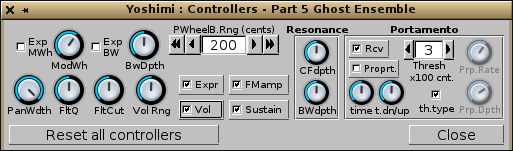
\includegraphics[scale=1.0]{2.0/Controllers.png}
   \caption{Controllers Dialog}
   \label{fig:controllers_dialog}
\end{figure}

   \begin{enumber}
      \item \textbf{Exp MWh}
      \item \textbf{ModWh}
      \item \textbf{Exp BW}
      \item \textbf{BwDepth}
      \item \textbf{PanWdth}
      \item \textbf{FltQ}
      \item \textbf{FitCut}
      \item \textbf{Vol Rng}
      \item \textbf{PWheelB.Rng}
      \item \textbf{Expr}
      \item \textbf{Breath} (1.5.6)
      \item \textbf{FMamp}
      \item \textbf{Vol}
      \item \textbf{Sustain}
      \item \textbf{Resonance} (section)
      \item \textbf{PortaMento} (section)
      \item \textbf{Reset all controllers}
      \item \textbf{Aftertouch}
      \item \textbf{Close}
   \end{enumber}

   \setcounter{ItemCounter}{0}      % Reset the ItemCounter for this list.

   \itempar{Exp MWh}{controllers!expression mod wheel}
   Exponential Modulation Wheel.
   Changes the modulation scale to exponential.

   Values: \texttt{Off*, On}

   \itempar{ModWh}{controllers!mod wheel depth}
   Modulation Wheel Depth.

   Values: \texttt{0 to 127, 80*}

   \itempar{Exp BW}{controllers!exp bandwidth controller}
   Exponential Bandwidth Controller.
   Changes the bandwidth scale to exponential.

   Values: \texttt{Off*, On}

   \itempar{BwDepth}{controllers!bandwidth depth}
   Bandwidth Depth.

   Values: \texttt{0 to 127, 64*}

   \itempar{Exp BW}{controllers!bandwidth depth}
   Exponential Bandwidth.
   Changes the bandwidth scale to exponential.

   Values: \texttt{0 to 127, 64*}

   \itempar{PanDpth}{controllers!panning depth}
   Panning Depth.

   Values: \texttt{0 to 64*}

   \itempar{FltQ}{controllers!filter Q depth}
   Filter Q (resonance) Depth.

   Values: \texttt{0 to 127, 64*}

   \itempar{FltCut}{controllers!filter cutoff depth}
   Filter Cutoff Frequency Depth.

   Values: \texttt{0 to 127, 64*}

   \itempar{Vol Rng}{controllers!volume range}
   Volume Range.

   Values: \texttt{64 to 127, 64*}

   \itempar{PWheelB.Rng}{controllers!pitch wheel range}
   Pitch Wheel Bend Range (cents).
   100 cents = 1 halftone.

   Values: \texttt{-6400 to 6400, 200*}

   \itempar{Expr}{controllers!expression}
   Expression Enable.
   Enable/disable expression.

   Values: \texttt{Off, On*}

   \itempar{Breath}{controllers!breath}
   Breath.

   Breath control was once a "per part" setting, but now it is a
   "per instrument" setting.  By default, this setting is enabled.
   This new switch is visible from version 1.5.6 on, and it is saved only in
   new \texttt{.xiy} format.
   See \sectionref{sec:configuration} for details on the new format.

   Values: \texttt{Off, On*}

   \itempar{FMamp}{controllers!fm amplitude}
   FM Amplitude Enable.
   Enable/disable receiving Modulation Amplitude controller (76).

   Values: \texttt{Off, On*}

   \itempar{Vol}{controllers!volume enable}
   Volume Enable.

   Values: \texttt{Off, On*}

   Enable/disable receiving volume controller.
   Sensitivity to MIDI volume change (CC7) is now variable in 'Controllers'
   in the same way as pan width etc. The numeric range is 64 to 127; the
   default at 96 gives the same sensitivity as before at -12dB relative to
   the GUI controls. 127 gives 0dB and 64 gives -26dB

   \itempar{Sustain}{controllers!sustain pedal enable}
   Sustain Pedal Enable.
   Enable/disable sustain pedal.

   Values: \texttt{Off, On*}

   \itempar{Reset all controllers}{controllers!reset all}
   Reset All Controllers.

   \itempar{Aftertouch}{controllers!aftertouch}
   Open Aftertouch window.

   \itempar{Close}{controllers!close}
   Close Window.

\subsubsection{Bottom Panel / Controllers / Aftertouch}
\label{subsubsec:bottom_panel_controllers_aftertouch}

   Completely new to \textsl{Yoshimi V 1.7.1}. Clicking on the button
   in \textbf{Controllers} opens the window below.

\begin{figure}[H]
   \centering
   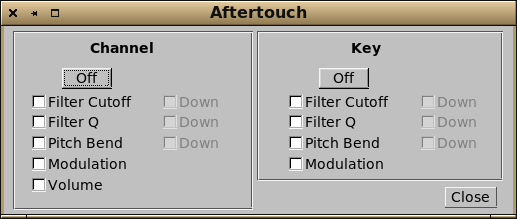
\includegraphics[scale=0.8]{2.0/AfterTouch.png}
   \caption{The MIDI Aftertouch Window}
   \label{fig:instrument_midi_aftertouch}
\end{figure}

This feature is so new that it may well change dependent on user feedback.

Both types of aftertouch are supported, \textsl{Channel} and \textsl{Key}. Many
keyboards only have \textsl{Channel} aftertouch , but \textsl{Key} is becoming
more common. \textsl{Key} is where the aftertouch
behaviour only affects the note produced by the key being pressed harder.

Currently, both forms support \textbf{Filter Cutoff} point,
\textbf{Filter Q}, and
\textbf{Pitch Bend}. Also note the extra checkboxes where these can be set to
move the controls down instead of up.

Also there is \textbf{Modulation}, and finally, \textbf{Volume} is only available
to \textbf{Channel} pressure.

One can have multiple actions such as
\textbf{Filter Q} and \textbf{Pitch Bend},
but one cannot have the same control on both
\textbf{Channel} and \textbf{Key}.

\subsubsection{Bottom Panel / Controllers / MIDI Controls}
\label{subsubsec:bottom_panel_controllers_midi_controls}

   There is a new button in the main window for access to the small MIDI CCs
   window. Access to this window used to require a right click on the
   Controllers button, but many people never knew it was available!  These
   controls can be used when one doesn't have a MIDI source connected, and they
   can also be learned and combined with others for greater expression.  This
   window has five controls that are MIDI-learnable.

\begin{figure}[H]
   \centering
   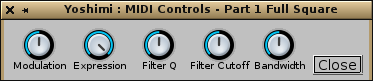
\includegraphics[scale=1.0]{1.5.4/MIDIcontrols.png}
   \caption{MIDI Controls from MIDI CCs Button}
   \label{fig:instrument_midi_controllers}
\end{figure}

   \begin{enumber}
      \item \textbf{Modulation}
      \item \textbf{Expression}
      \item \textbf{Filter Q}
      \item \textbf{Filter Cutoff}
      \item \textbf{Bandwidth}
   \end{enumber}

   \setcounter{ItemCounter}{0}      % Reset the ItemCounter for this list.

   Will has one keyboard that sends aftertouch messages, and all of these work
   correctly with it. An interesting effect was to have a sawtooth wave set up
   in \textbf{AddSynth} and the frequency LFO level turned up.  Then, he
   learned \textbf{Modulation}, \textbf{Expression}, and \textbf{Filter
   Cutoff}, all on aftertouch. He then reduced their ranges in the MIDI learn
   window and the effect was very interesting.  Try it!

   Because of the way this is implemented, these controls are also accessible
   via CLI direct access for both for read and write, and the knobs will
   respond to this, as well as to learned controls.

   \itempar{Modulation}{controllers!modulation}
   Affects the (amplitude) modulation of all engines in the part.

   \itempar{Expression}{controllers!expression}
   Affects the "expression" of all engines in the part.

   \itempar{Filter Q}{controllers!filter Q}
   Affects the sharpness of the filtering of all engines in the part.

   \itempar{Filter Cutoff}{controllers!filter cutoff}
   \index{brightness}
   Affects the brightness of all engines in the part by increasing or reducing
   the corner frequency.

   \itempar{Bandwidth}{controllers!bandwidth}
   \index{Master Bandwidth}
   The master bandwidth control affects all engines in a part, and is
   real-time. It is also highly dependent on the harmonic structure, so is most
   effective on SubSynth sounds.  Like all of these MIDI controls, it is a part
   control, not an instrument setting, and is never saved.
   It is available in the window shown above, the command-line,
   and it is learnable.
   It considerably "expands" some instruments.

\subsubsection{Bottom Panel / Controllers / Resonance}
\label{subsubsec:bottom_panel_controllers_resonance}

   \setcounter{ItemCounter}{0}      % Reset the ItemCounter for this list.

   \itempar{CFdepth}{controllers!resonance CF depth}
   Resonance Center Frequency Depth,
   Center Frequency Controller Depth.

   Values: \texttt{0 to 127, 64*}

   \itempar{BWdepth}{controllers!resonance BW depth}
   Resonance Bandwidth Depth,
   Resonance Bandwidth Controller Depth.

   Values: \texttt{0 to 127, 64*}

\subsubsection{Bottom Panel / Controllers / Portamento}
\label{subsubsec:bottom_panel_controllers_portamento}

   \setcounter{ItemCounter}{0}      % Reset the ItemCounter for this list.

   \itempar{Rcv}{controllers!portamento receive}
   Portamento Receive,
   Receive Portamento Controllers.
   Determines if the part receives Portamento On/Off (65) controller.

   Values: \texttt{Off, On*}

   \itempar{Proprt}{controllers!portamento proportional}
   Portamento Proportional,
   Enable Proportional Portamento (over fixed portamento).

   Values: \texttt{Off*, On}

   \itempar{time}{controllers!portamento time}
   Portamento time.
   The duration of the portamento.

   Values: \texttt{0 to 127, 64*}

   \itempar{t.dn/up}{controllers!portamento time, down/up}
   Portamento Time Stretch (up/down).

   Values: \texttt{0 to 127, 64*}

   \itempar{threshx100 cnt}{controllers!portamento threshold}
   Threshold of the Portamento.
   The minimum or maximum difference of notes in order
   to do the portamento (x 100 cents).
   It represents the minimum or the maximum number of halftones (or hundred
   cents) required to start the portamento. The difference is computed
   between the last note and current note.
   The threshold refers to the frequencies and \textsl{not} to MIDI notes (one
   should consider this if one uses microtonal scales).

   Values: \texttt{0 to 127, 3*}

   \itempar{th.type}{controllers!portamento threshold type}
   Threshold Type (min/max).
   Checked means that the portamento activates when the difference of
   frequencies is above the threshold ("thresh"); not checked is for below
   the threshold.

   Values: \texttt{Off, On*}

   \itempar{Propt}{controllers!portamento proportional}
   Proportional Portamento.
   If set, the portamento is proportional to ratio of frequencies.

   Values: \texttt{Off, On*}

   \itempar{Prp.Rate}{controllers!portamento rate}
   Distance required to double change from nonproportional
   portamento time.
   The ratio needed to double the time of portamento.

   Values: \texttt{0 to 127, 80*}, requires \textbf{Proprt.} = \texttt{On}

   \itempar{Prp.Depth}{controllers!portamento depth}
   The difference from nonproportional portamento.

   Values: \texttt{0 to 127, 90*}, requires \textbf{Proprt.} = \texttt{On}

\subsection{Bottom Panel Instrument Edit}
\label{subsec:bottom_panel_instrument_edit}

   The main instrument-editing ("part edit")
   dialog is relatively simple, and provides for
   editing information that identifies the instrument, and buttons to access
   the more complex dialogs of the
   \textbf{ADDsynth}, \textbf{SUBsynth}, \textbf{PADsynth}, \textbf{Kit Edit},
   and \textbf{Effects} components.


\begin{figure}[H]
   \centering
%  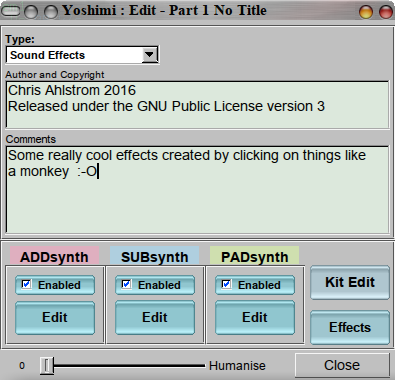
\includegraphics[scale=1.0]{1.3.9/edit-instrument.png}
%  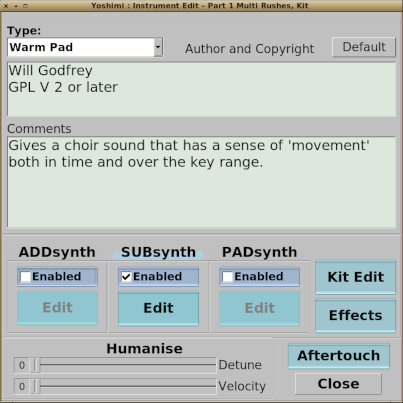
\includegraphics[scale=1.0]{2.0/PartEdit.png}
   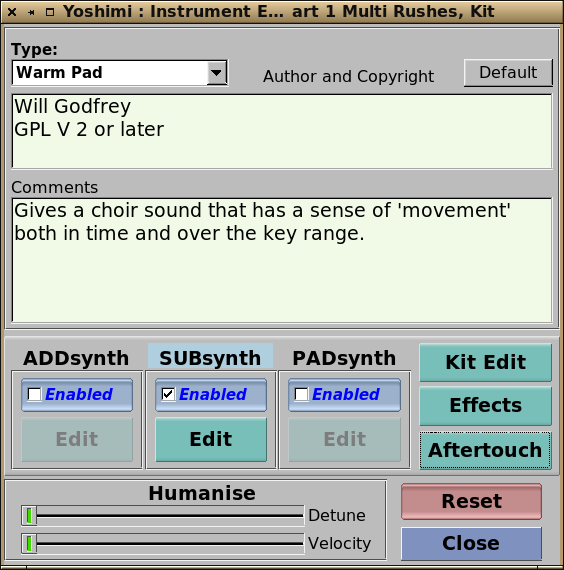
\includegraphics[scale=0.5]{2.1.2/edit.png}
   \caption{Part Edit (Instrument) Dialog}
   \label{fig:instrument_edit_dialog}
\end{figure}

   This dialog provides a very broad overview of the instrument, and
   provides access to far more detailed dialogs to edit the instrument.
   This dialog is called up by the \textbf{Edit} button on the bottom panel
   of the main \textsl{Yoshimi} main screen.

   \begin{enumber}
      \item \textbf{Type}
      \item \textbf{Author and Copyright}
      \item \textbf{Default}
      \item \textbf{Comments}
      \item \textbf{ADDsynth}
      \begin{enumber}
         \item \textbf{Enabled}
         \item \textbf{Edit}
      \end{enumber}
      \item \textbf{SUBsynth}
      \begin{enumber}
         \item \textbf{Enabled}
         \item \textbf{Edit}
      \end{enumber}
      \item \textbf{PADsynth}
      \begin{enumber}
         \item \textbf{Enabled}
         \item \textbf{Edit}
      \end{enumber}
      \item \textbf{Kit Edit}
      \item \textbf{Effects}
      \item \textbf{Aftertouch}
      \item \textbf{Detune}, slider, part of the extended \textbf{Humanise}.
      \item \textbf{Velocity}, slider, part of the extended \textbf{Humanise}.
      \item \textbf{Close}
   \end{enumber}

   The \textbf{ADDsynth}, \textbf{SUBsynth}, \textbf{PADsynth},
   \textbf{Kit Edit}, and \textbf{Effects}
   dialogs are detailed in separated sections, as they are all
   very complex dialogs with many sub-dialogs.

   \setcounter{ItemCounter}{0}      % Reset the ItemCounter for this list.

   \itempar{Type}{edit!category}
   Instrument Type.
   Instrument Category.

   This dropdown dialog allows one to tag the type of instrument, to
   indicate what category of instruments it fits into.
   The following figure shows the types.

\begin{figure}[H]
   \centering
   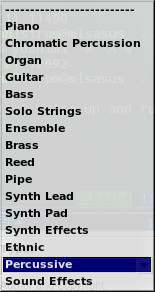
\includegraphics[scale=1.0]{bottom-panel/edit-instrument-type.jpg}
   \caption{Instrument Type Drop-down List}
   \label{fig:instrument_type_dropdown}
\end{figure}

   Values: \texttt{Piano, Chromatic Percussion, Organ, Guitar, Bass,
              Solo Strings, Ensemble, Brass, Reed, Pipe,
              Synth Lead, Synth Pad, Synth Effects, Ethnic,
              Percussive, Sound Effects}

   \itempar{Author and Copyright}{edit!author/copyright}
   This field provides space for identifying the author, copyright, and
   license for the part.  Starting text can be saved by using the
   \textbf{Default} button, described in the next section.

   \itempar{Default}{edit!default}
   In the main part \textbf{Instrument Edit} window there is a new
   \textbf{Default} button at top right.
   We hope this encourages people
   to fill in the Author and Copyright information.
   To set it up, fill in the text field as normal,
   then, while holding down the Ctrl key, click on the button
   (left or middle mouse click) . This text will now be stored in
   one's \textsl{Yoshimi} configuration directory,
   and whenever one creates a new instrument, just
   click on the \textbf{Default} button, and the saved text will be
   filled in.

   This button was added to discourage users from adding supplementary
   information directly into the bank directories.

   \itempar{Comments}{edit!comments}
   Allows free-form comments and notes to be entered.

   \itempar{ADDsynth}{edit!addsynth}

   \begin{enumber}
      \item \textbf{Enabled}.
      Enables this synth type to be used in the part/instrument.
      When enabled, its marker colour, red, is shown.
      \item \textbf{Edit}.
      Brings up the editing dialog presented in
      \figureref{fig:addsynth_edit_dialog}.
      There one will find a full discussion of that dialog.
   \end{enumber}

   \itempar{SUBsynth}{edit!subsynth}

   \begin{enumber}
      \item \textbf{Enabled}.
      Enables this synth type to be used in the part/instrument.
      When enabled, its marker colour, blue, is shown.
      \item \textbf{Edit}.
      Brings up the editing dialog presented in
      \figureref{fig:subsynth_edit_dialog}.
      There one will find a full discussion of that dialog.
   \end{enumber}

   \itempar{PADsynth}{edit!padsynth}

   \begin{enumber}
      \item \textbf{Enabled}.
      Enables this synth type to be used in the part/instrument.
      When enabled, its marker colour, green, is shown.
      \item \textbf{Edit}.
      Brings up the editing dialog presented in
      \figureref{fig:padsynth_edit_dialog}.
      There one will find a full discussion of that dialog.
   \end{enumber}

   \itempar{Kit Edit}{edit!kit}
   Brings up the editing dialog presented in
   \figureref{fig:kit_edit_dialog}.
   There one will find a full discussion of that dialog.

   \itempar{Effects}{edit!effects}
   Brings up the editing dialog presented in
   \figureref{fig:effects_edit_none}.
   There one will find a full discussion of that dialog.

   When the effects panels are brought up from this button, there are two extra
   user-interface elements:
   \index{effects!bypass}
   \textbf{Bypass} and \textbf{Close}.
   If the \textbf{Bypass} item is checked, then the effect is not
   used; it is taken out of the circuit.

   \itempar{Aftertouch}{controllers!aftertouch}
   Open Aftertouch window.

   \itempar{Detune (Humanise)}{edit!detune}
   Small Random Detune.
   \index{Humanise}
   \index{edit!detune}

   \itempar{Velocity (Humanise)}{edit!velocity}
   Small Random Velocity Attenuation.
   \index{Humanise}
   \index{edit!velocity}

   There used to be a single Humanise control which set a random detune in cents.
   Since \textsl{Yoshimi} V 1.6.0 this has become the detune component of Humanise.

   The velocity slider gives an independent random attenuation as a percentage of
   the full output. This, as well as changing the perceived volume, will change any
   velocity sensing features, such as filters.

   Combined, they lend considerable complexity or piquancy to the part. Both have the same
   numeric range.

   Values: \texttt{0* to 50}

   \itempar{Close}{edit!close}
   Closes the Edit window.

%-------------------------------------------------------------------------------
% vim: ts=3 sw=3 et ft=tex
%-------------------------------------------------------------------------------
